\documentclass[tikz]{standalone}
\usepackage{fixltx2e}%  http://ctan.org/pkg/fixltx2e

\usepackage[utf8]{inputenx}%  http://ctan.org/pkg/inputenx
% Euler for math | Palatino for rm | Helvetica for ss | Courier for tt
\renewcommand{\rmdefault}{ppl}% rm
\linespread{1.05}% Palatino needs more leading
\usepackage[scaled]{helvet}% ss //  http://ctan.org/pkg/helvet
\usepackage{courier}% tt // http://ctan.org/pkg/courier
\usepackage{eulervm}  %  http://ctan.org/pkg/eulervm
% a better implementation of the euler package (not in gwTeX)
\normalfont%
\usepackage[T1]{fontenc}%  http://ctan.org/pkg/fontenc
\usepackage{textcomp}%  http://ctan.org/pkg/textcomp
\begin{document}

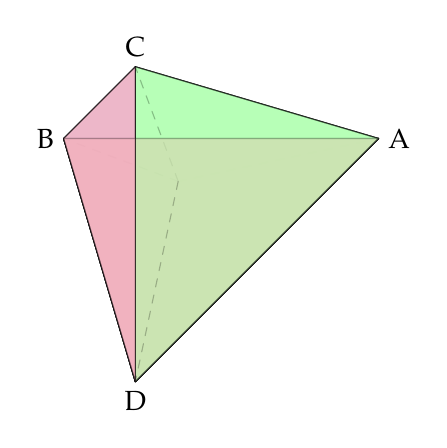
\begin{tikzpicture}[line join = round, line cap = round]
\pgfmathsetmacro{\factor}{1/sqrt(2)};
\coordinate [label = right:A] (A) at (2, 0, -2*\factor);
\coordinate [label = left:B]  (B) at (-2, 0, -2*\factor);
\coordinate [label = above:C] (C) at (0, 2, 2*\factor);
\coordinate [label = below:D] (D) at (0, -2, 2*\factor);

%\draw[->] (0,0) -- (3,0,0) node[right] {$x$};
%\draw[->] (0,0) -- (0,3,0) node[above] {$y$};
%\draw[->] (0,0) -- (0,0,3) node[below left] {$z$};
\foreach \i in {A, B, C, D}{
  \draw[dashed] (0, 0) -- (\i);
  \draw[-, fill = red!30, opacity = .5] (A) -- (D) -- (B) --cycle;
  \draw[-, fill = green!30, opacity = .5] (A) -- (D) -- (C) --cycle;
  \draw[-, fill = purple!30, opacity = .5] (B) -- (D) -- (C) --cycle;
}
\end{tikzpicture}

\end{document}
%%% Local Variables:
%%% mode: latex
%%% TeX-master: t
%%% End:
